% !TeX spellcheck = de_DE 
\chapter{Implementierung}
\label{sec:imp}
In meiner Abschlussarbeit präsentiere ich die praktische Lösung für das PSE-Labor der Beuth Hochschule für Technik Berlin. Die gesamte Aufgabe lässt sich in drei Bestandteile unterteilen: Register-Client, Server und Display-Client. Erstens wird Register-Client implementiert, damit wird RFID Leser am Raspberry Pi Mikrocomputer angeschlossen, alle Treiber installiert und auf Python Programmierung Sprache die Software geschrieben, die die ständige Überwachung des empfangenden von RFID Leser Daten zulässt und die Verbindung mit dem Server zulässt. Falls die empfangene Daten korrekt sind, d.h.  eine richtige MIFARE Studentenkarte oder einen richtigen RFID-Transponder abgelesen wurde, schickt die Software die abgelesene Daten zum Server ab. Der Server ist der zweite Bestandteil der Abschlussarbeit und wird mit Hilfe Django Framework, Django Finite State Machine auf Python Programming Sprache implementiert. Server enthält die Datenbank mit die Datensätzen über die alle im PSE-Labor vorhandenen ausleihenden Boards, die zum Modul im laufenden Semester registrierten Studenten und  geschehenen Ausleihe/Rückgabe-Vorgänge. Es wird von Server überprüft, ob eine von Register-Client abgelesene Studentenkarte einem zugelassenen für die Ausleihe Student gehört und die entsprechenden Information auf Display-Client geschickt. Es wird auch von Server bestätigt, ob für die Ausleihe/Rückgabe neben dem RFID-Leser gehaltenen Raspi Board dem Student ausgeliehen/vom Student zurückgegeben werden darf. Darauf aufbauend, wird der dritte Teil namens ein Display-Client als dynamische HTML-Seite realisiert, die eine Verbindung zum Server Mithilfe des HTTP-Protokolls und eingebauten im Browser Kommunikationsmittel die asynchrone Nachrichten zu schicken, bereitstellt. Für die dynamische Aktualisierung des Inhalts der Webseite und einen Zugang zum asynchronen HTTP-Client wird jQuery benutzt.
\section{Register-Client}
\label{sec:register_client}
Das folgende Kapitel beschäftigt sich mit der Implementierung des Register-Client auf Raspberry Pi Board mit angeschlossenen RFID-Leser. Dieser Teil der verteilte System lässt sich wie folgendes unterteilen. Zuerst wurde das Betriebssystem Raspbian auf Board zum Leben gebracht und dann die alle notwendigen für RFID-Leser Treiber installiert. Nach dem der RFID-Leser funktionieren angefangen und die Daten von RFID-Transponder abgelesen hat, wurde die nächste Herausforderungen gelöst: die Struktur die zu empfangenen Daten wurde verstanden, richtig bearbeitet, eine JSON-Datei erstellt und durch die HTTP-Protokoll dem Server geliefert. 

\subsection{Installation des Betriebssystem}
\label{sec:register_client:raspbian}
Der vorhandene für die Abschlussarbeit Raspberry Pi 3 Model B+ wurde nicht als Starter Kit mir übergeben, dann wurde es zusätzlich benötigt\cite[pp. 21-22]{gareth:raspi}: 
\begin{itemize}
	\item \textbf{USB-Netzteil} mit einer Nennleistung von 2,5 A (2,5 A) oder 12,5 Watt (12,5 W) und einem Micro-USB-Anschluss. 
	\item \textbf{microSD-Karte}, die als permanenter Speicher des Raspberry Pi dient; Alle von Benutzer erstellten Dateien und die installierte Software sowie das Betriebssystem selbst werden auf der microSD-Karte gespeichert.
	\item \textbf{USB-Tastatur und -Maus}, mit denen den Raspberry Pi gesteuert werden kann. Fast jede kabelgebundene oder kabellose Tastatur und Maus mit USB-Anschluss funktioniert mit dem Raspberry Pi.
	\item \textbf{Das HDMI-Kabel}, das Ton und Bilder vom Raspberry Pi auf Fernseher oder Monitor überträgt. Sie müssen nicht viel Geld für ein HDMI-Kabel ausgeben. 
\end{itemize}

Die Arbeit mit einem RaspberryPi setzt ein paar Anfangsinvestitionen voraus, die auch von den angestrebten Aufgaben und Projekten abhängen. Zuerst gäbe es die Möglichkeiten, dass der gekaufte Raspberry Pi Board bereits ein Betriebssystem darauf installiert hätte. Aber es war nicht der Fall von vorhandenen im PSE-Labor Board. Um ein Betriebssystem auf diesen Raspberry Pi zu bringen, muss eine SD-Karte mit einem Betriebssystem-Image "geflasht" werden. Dafür zunächst wurde die Distribution von der Website Raspbian.org herunterladen und die MicroSD-Karte in den Kartenleser eines vorhandenen im PSE-Labor PC eingelegt. Anschließend wurde mit dem Macintosh Disk Utility-Dienstprogramm das heruntergeladene und entpackte Betriebssystem für den RaspberryPi auf eine Speicherkarte geschrieben. Dann ist die Karte in Raspberry Pi einzulegen. Der Raspi ist damit betriebsbereit und muss für die zukünftigen Anwendungen noch konfiguriert werden. Wenn der Pi zum ersten Mal eingeschaltet wird, wird viel Text auf dem Bildschirm angezeigt. Diese werden als Startmeldungen bezeichnet. Wenn Raspbian zum ersten Mal gestartet wurde, kann es ein oder zwei Minuten dauern, um die Nutzung des freien Speicherplatzes auf der microSD-Karte optimal anzupassen. Beim nächsten Start geht es schneller. Schließlich ist kurz ein Fenster mit dem Raspberry Pi-Logo zu sehen, dann wird Terminal Fenster angezeigt, in dem es einloggt werden muss. Zum ersten Einloggen wird den Standardbenutzername "pi" und das Standardkennwort  "raspberry" verwendet. Um Register-Client vor sowohl Online-Bedrohungen als auch von Missbrauch im Labor zu schützen, wurde das Standardkennwort sofort geändert. Der nächste Schritt ist Raspbian bis zur Version "Raspbian mit dem Raspberry Pi Desktop" zu aktualisieren, damit die grafische Benutzeroberfläche und Chromium Browser zu Verfügung stehen können. Dies kann mit dem Terminalbefehl gemacht werden:
\begin{lstlisting}
sudo apt-get install lxde-core xserver-xorg xinit
\end{lstlisting}
Dann ist der Raspberry Pi erneut zu laden. Nachdem Raspberry Pi-Logo wieder angezeigt wurde, wäre der Raspbian-Desktop zu sehen. Somit gilt Betriebssystem als vollständig installiert und kann benutzt werden. Das war aber nicht der Fall mit dem vorhandenen Hardware, da es plötzlich eine Boot-Schleife vorkam, nachdem der Mikrocomputer eingeschaltet wurde und der Startvorgang nicht abgeschlossen werden konnte. Anstatt das zum Benutzung bereiteten Betriebssystem mit der grafische Benutzeroberfläche zu sehen,  wird eine Schleife erzeugt, in der die Startvorgang kontinuierlich und wiederholt ausgeführt wurde und somit eine Nutzung der Mikrocomputers unmöglich ist. Nach den mehreren Recherchen wurde es vermutet, dass es durch eine unzureichende Stromversorgung verursacht werden könnte. Es wurde aber zuerst nicht versucht, einen USB-Netzteil zu wechseln, da die anderen USB-Netzteil man durch PSE-Labor bestellen und eine Zeit abwarten muss. Jedoch wurde eine erzeugte Boot-Schleife mit einem anderen Terminalbefehl erfolgreich gelöst:
\begin{lstlisting}
sudo apt-get install --reinstall pcmanfm
\end{lstlisting}
Bei der Arbeit mit dem Mikrocomputer tritt jedoch später ein Problem mit der Stromversorgung auf. Der Fall kann im entsprechenden Kapitel \ref{sec:register_client:voltage_issue} nachgelesen werden.


\subsection{Installation der Treibers für RFID-Leser}
\label{sec:register_client:install_rfid}
Im weiteren Verlauf der Arbeit wird den RFID Leser/Schreiber ACR122U erfolgreich angefahren, der auf der Basis der 13,56 MHz kontaktlosen (RFID ) Technologie entwickelt wurde. Der ACR122U USB Kartenleser unterstützt nicht nur Mifare ® Technologien, sondern auch alle vier Typen von NFC -Tags. Diese Anforderung ist für vorliegende Abschlussarbeit wichtig, da Studierenden-Ausweise der Beuth Hochschule mit dieser Technologie gelesen werden können. Obwohl Raspbian mit einer Reihe von Software vorinstalliert ist, wird es aber zusätzlich benötigt, die Treiber für RFID-Leser zu installieren. Es sollte an dieser Stelle auch noch angemerkt werden, dass am Anfang der Entwicklungsprozess ein anderen RFID-Leser angeschlossen wurde als der, den in der Abschlussarbeit zu beschreiben und zu beobachten ist. Zuerst wurde die Treiber für Reiner SCT CyberJack RFID Basis\cite{website:4} installiert. Die Schritte sollten in der Abschlussarbeit nicht unerwähnt bleiben, da die damals für den ersten RFID-Leser installierte Treiber und Daemons (Appendix \ref{sec:appendix:daemon}) wurden endlich für den zweiten RFID-Leser benutzt, mit dem die Entwicklung der Aufgabe abgeschlossen wurde. Der Grund für die Hardwareaustausch ist die festgestellte Tatsache, dass Reiner SCT CyberJack RFID Leser die Studentenkarten nicht ablesen konnte. Obwohl in der Spezifikation es steht, dass die Reiner RFID-Leser kontaktlose RFID Chipkarten wie eID mit dem neuen Personalausweis (nPA), GeldKarte oder eTicketing unterstützt, wurde es unmöglich mit den MIFARE-Transponder 13,561 MHz Funkbereich ins Spiel zu bringen. Die Studierenden-Ausweise der Beuth sollten mit dieser Technologie gelesen werden und somit ist diese Anforderung für die vorliegende Abschlussarbeit wichtig. 

Um RFID-Leser anzuschließen, muss man den Leser über USB mit einem Raspberry Pi verbunden. Der Typ des RFID-Lesegeräts, der für die vorliegende Abschlussarbeit verwendet wird, ist ein ACR122U-A9 von Advanced Card Systems\cite{website:7}, den auf der Abbildung\ref{fig:rfid_hard} zu sehen. Zuerst müssen wir die Paketlisten aktualisieren und einige Pakete herunterladen und installieren:\cite{website:6}. Die folgenden Abhängigkeiten werden benötigt im System mit dem Befehl "sudo apt-get install" zu installieren: $libusb-dev, libpcsclite-dev, libpcsclite1, libccid, pcscd, pcsc-tools, libpcsc-perl, libusb-1.0-0-dev, libtool, libssl-dev$.\\
\begin{wrapfigure}{l}{0.45\textwidth}
	\fbox{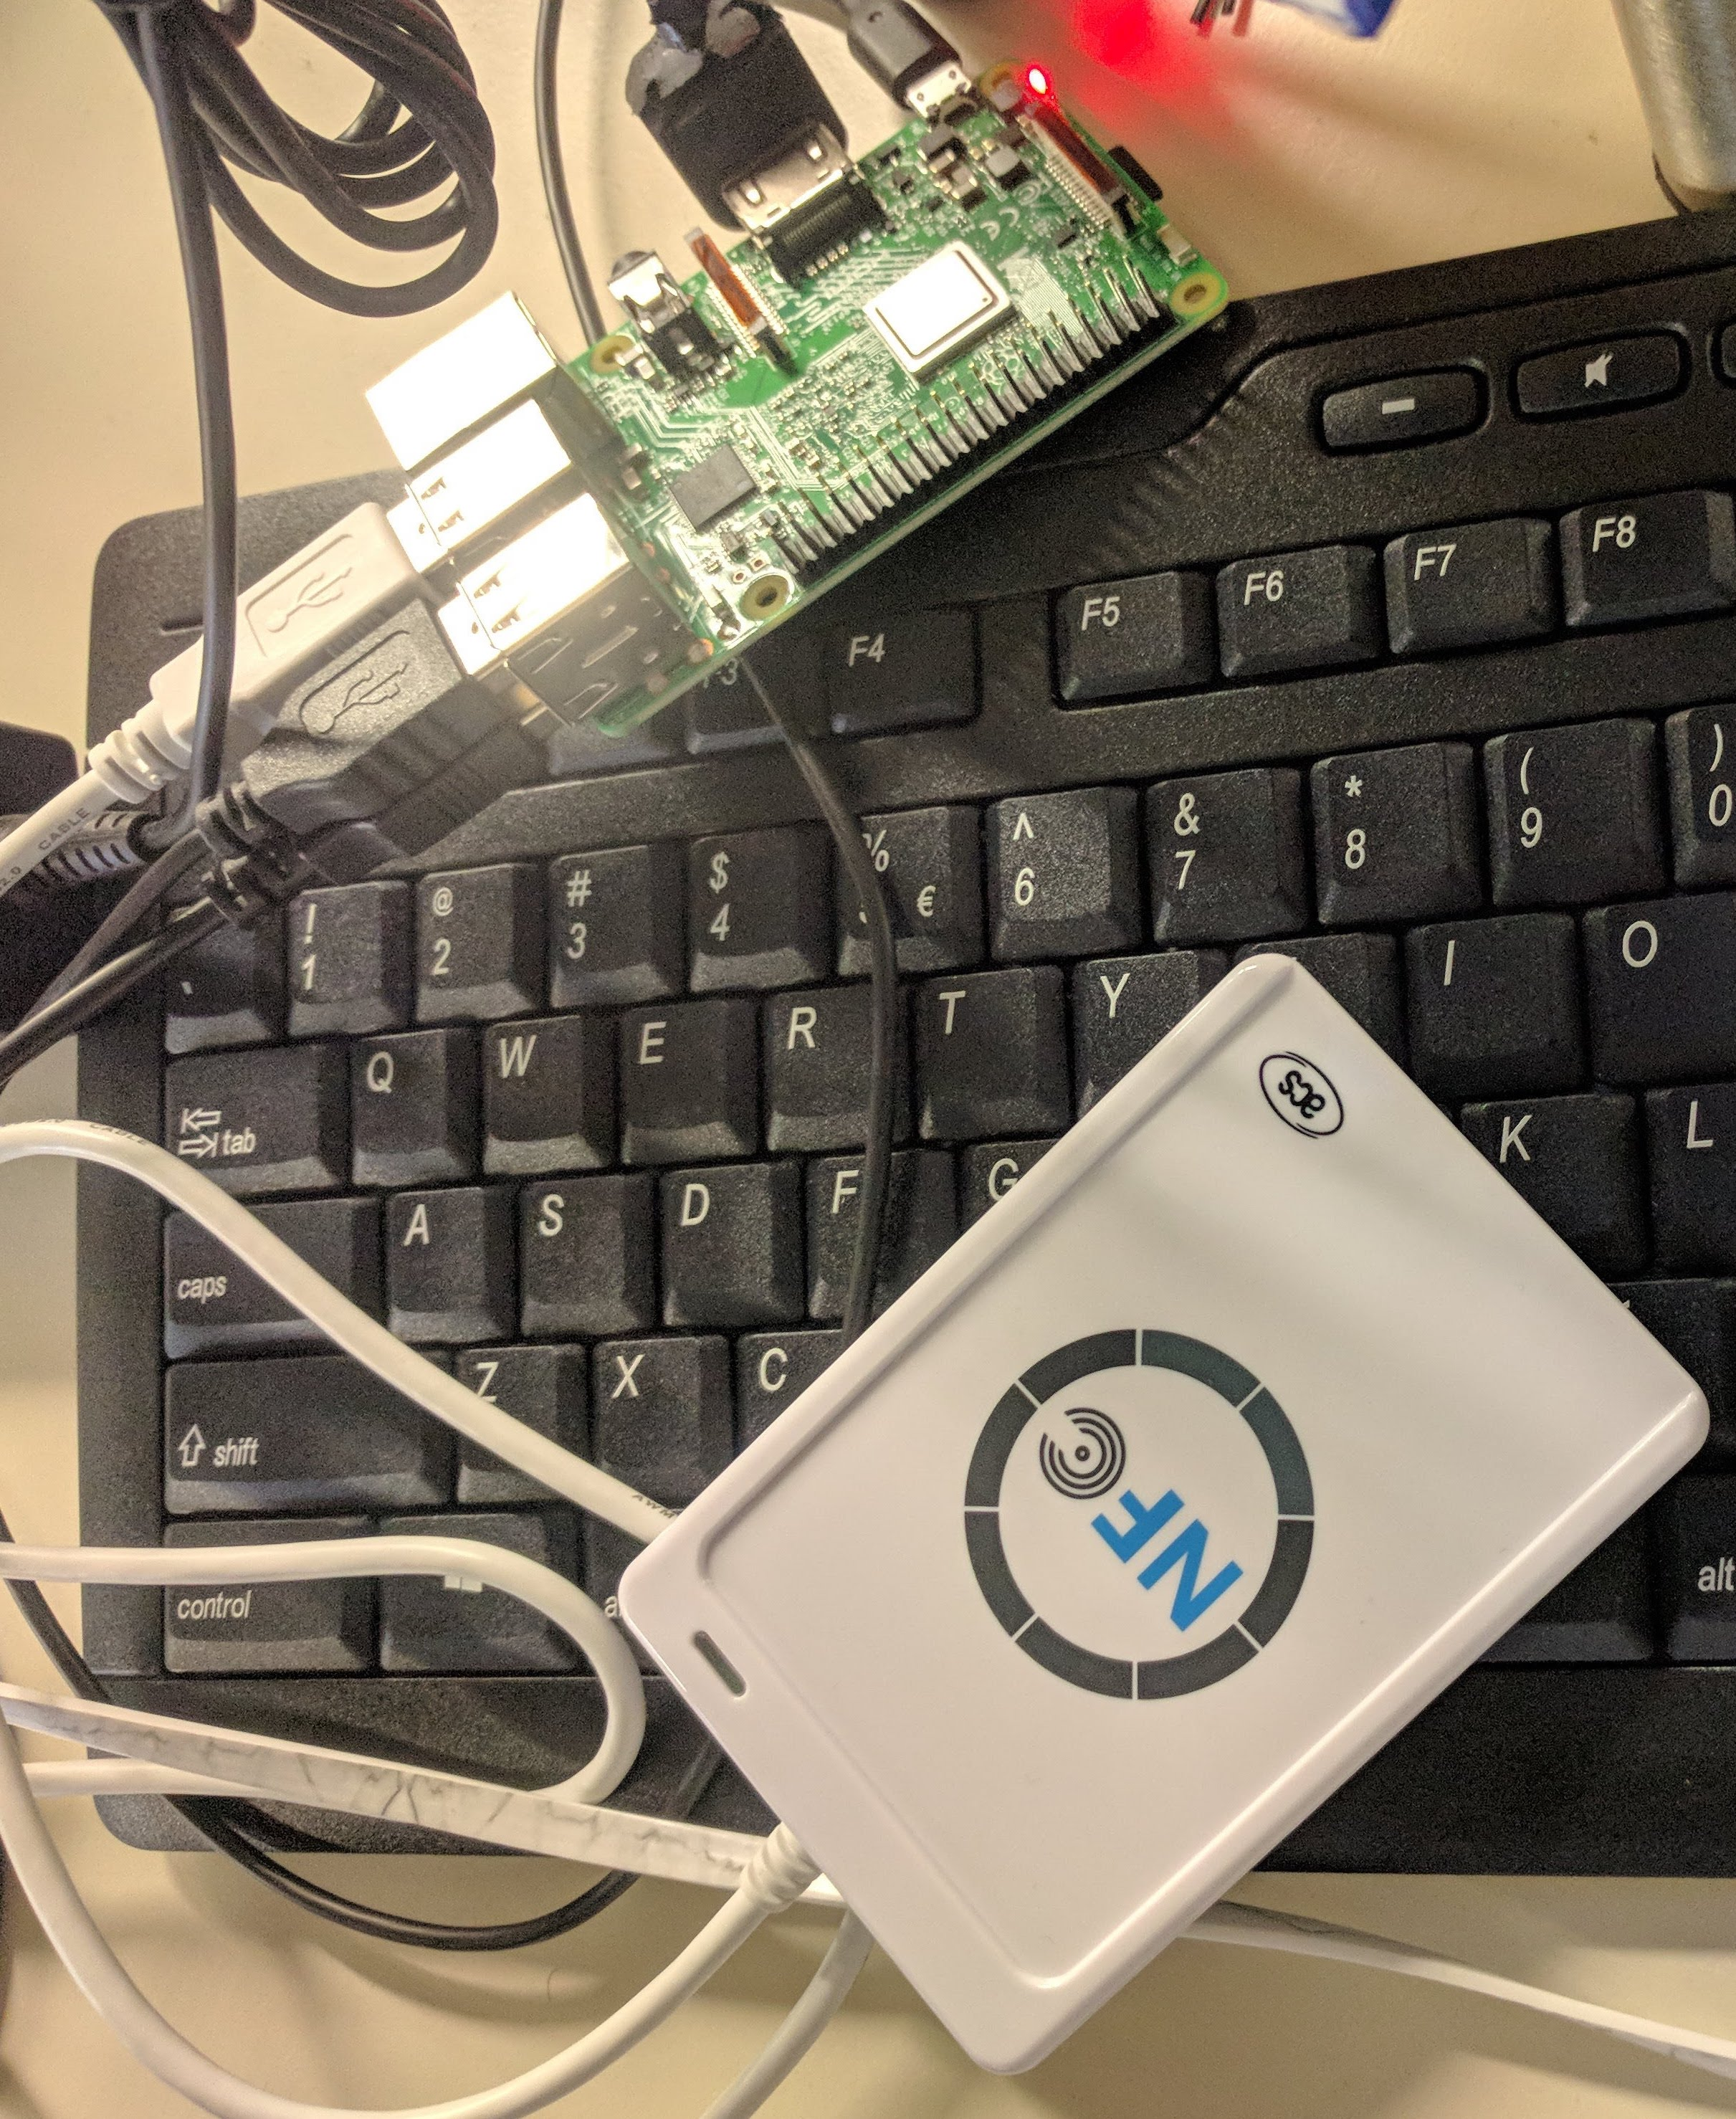
\includegraphics[width=0.42\textwidth]{gfx/rfid_hard.jpg}}
	\caption{ACR122U-A9 von Advanced Card Systems und Raspbery Pi}
	\label{fig:rfid_hard}
\end{wrapfigure}
PC/SC ist ein Standard für die Schnittstelle von Computern mit Smartcards, der auf den meisten Betriebssystemen, einschließlich Windows und Linux, verfügbar ist. PC/SC-Kopplungsgeräte benötigen einen Treiber, mit dem Anwendungen die Karte einfach erreichen können. Da PC/SC für Smartcards entwickelt wurde - und in einer Zeit, in der Smartcards nur Kontaktkarten waren funktioniert es auch mit den kontaktlosen Karten, falls RFID-Leser es unterstützt. Das Daemon-Programm für pcsc-lite namens pcscd koordiniert die Kommunikation mit Smartcard-Lesegeräten und Smartcards sowie kryptografischen Tokens, die mit dem System verbunden sind. Normalerweise wird pcscd beim Booten von /etc/init.d/pcscd gestartet. Damit können Anwendungen auf Smartcards und Lesegeräte zugreifen, ohne die Details der Karte oder des Lesegeräts zu kennen. Das Laden von Treibern für Kartenleser wird von pcscd koordiniert. Der Zweck von pcsc-lite besteht darin, eine kompatible API (Winscard) für die Migration von Windows-basierten PC / SC-Anwendungen auf Unix bereitzustellen\cite{website:5}. Die allgemeinen Zugriff auf USB-Geräte bietet eine C-Bibliothek namens libusb.  Sie soll von Entwicklern verwendet werden, um die Produktion von Anwendungen zu erleichtern, die mit USB-Hardware kommunizieren. Es ist portabel, da mit einer einzigen plattformübergreifenden API auf USB-Geräte unter Linux, MacOS, Windows usw. zugegriffen werden kann. Sie wird im Benutzermodus ausgeführt und somit für die Kommunikation der Anwendung mit einem Gerät keine besonderen Berechtigungen oder Erhöhungen erforderlich sind.\cite{website:8}

Dann laden wir die Open-Source-Bibliothek libnfc für Near Field Communication (NFC) herunter, extrahieren, konfigurieren und installieren es. Nach der erfolgreichen Installation kann den verbindenden über USB RFID-Leser mithilfe des Tools lsusb angesehen werden: es wird VendorId und ProductID angezeigt. Es ist auch notwendig die abgelesene VendorId und ProductID in der entsprechenden XML-Datei. Die Datei auf der MicroSD-Karte ist zu finden :
\begin{lstlisting}
/usr/lib/pcsc/drivers/ifd-ccid.bundle/Contents/info.plist
\end{lstlisting}

\subsection{Spannungsproblem und Lösung}
\label{sec:register_client:voltage_issue}
Nachdem der RFID-Leser angeschlossen wurde, tritt es ein weiteres Problem, das die freie Benutzung der Raspberry Pi unmöglich macht. Es wird unabhängig von der Zeit und vorherigen Geschehen eine Fehlermeldung "under voltage detected (0x000050000000)". Es wird zuerst versucht die kabellose USB-Tastatur und -Maus abzuschalten. USB eine aktive Abfrage seine Ports (Polling) benötigt, was bedeutet, dass die Anzahl der für andere Aufgaben verfügbaren CPU Zyklen geringer ist. Dies kann dazu führen, dass die CPU-Frequenz ansteigt, wodurch der Stromverbrauch höher wäre. Es wurde festgestellt, dass mit unverbundenen USB-Tastatur und -Maus die Fehlermeldung trotzt vorkommt. Nur wenn der RFID-Leser angeschaltet wurde, kam es keine neue Fehlermeldung. Dann es wurde geprüft, ob ausgewählten RFID-Leser mit dem vorhandenen Mikrocomputer überhaupt kompatibel ist und nach der Lösung gesucht, mit der die zukünftige Entwicklung weiterlaufen kann.    

Anfänglich wurde als Spannungsversorgungsteil ein USB-Netzteil von einem modernem bei Autorin der Abschlussarbeit vorhandenen zu Hause Smartphone benutzt. Das offizielle Raspberry Pi-Netzteil ist die empfohlene in der Dokumentation Wahl, jedoch wurde zuerst mit dem Mikrocomputer nicht gekauft. Ein leistungsfähiger USB-Netzteil könnte den schnell wechselnden Strombedarf des Raspberry Pi bewältigen. Nach der Besprechung des Problems mit den PSE-Labor Mitarbeiter wurde ein Samsung USB-Netzteil gegen einen Anker USB-Netzteil ausgetauscht und festgestellt, dass das Spannungsproblem mit den verbundenen sowohl USB-Tastatur und -Maus als auch RFID-Leser während des Ablesevorgangs nicht wieder erscheint. 

\subsection{Python Programmierung des RFID-Lesers}
\label{sec:register_client:smart}
Nachdem es gelingt mir, die Hardware angefahren und die ersten Studentenkarte so abzulesen, dass es ein Schallton von RFID-Leser erzeugt wurde, sollte eine weitere Aufgabe gelöst werden: die Daten von RFID-Tag auf einem auszuleihenden Raspi Board von Studentenkarte unterscheiden zu können. Es sollte ausgeschlossen werden, dass ein Ausleihe-/Rückgabevorgang angefangen wird, falls eine falsche Studentenkarte (z.B. mit einer BVG Jahresfahrkarte) am RFID-Leser präsentiert wird. Als es im Kapitel \ref{sec:theorie:mifare} erklärt wurde, sind die neuen Campus Karte der Beuth Hoschule für Technik Berlin mit den die MIFARE-Transponder hergestellt. Für die Programmierung des RFID-Lesers wird Smartcard-Schnittstelle benutzt, deren Installierung geschah zusammen mit pyscard und im Kapitel \ref{sec:register_client:install_rfid} geschrieben. Diese Schnittstelle steht für den Entwickler für die Arbeit mit Smartcards und NFC-Geräten zur Verfügung, sie wird in Form mehrerer Systemdienste implementiert und ihr Schnittstellenteil ist das PC/SC-Framework. PC/SC steht für Personal Computer/Smart Card.

Es steht mehreren Möglichkeiten für die Entwicklung eine Sprache zu wählen: die Funktionen der Smartcard-Schnittstelle können mit Python, C/C++ und Java Sprache verwendet werden. Die Programmierung des Register-Clients wird auf Python Sprache gemacht, dieselbe Sprache wird für Server während der Arbeit mit Django Framework benutzt. Die Entwicklung mit dem Importieren der PCSC-Header-Dateien beginnt. 
\begin{lstlisting}
from smartcard.System import readers
from smartcard.ATR import ATR
from smartcard.CardMonitoring import CardMonitor, CardObserver
from smartcard.CardRequest import CardRequest
\end{lstlisting}
Wann eine RFID-Leser über USB angeschlossen wird, kann es eine Verbindung zur PC/ SC-Bibliothek hergestellt und eine Liste der verfügbaren Terminals abgerufen werden. Alle API-Funktionen geben einen Statuscode zurück. Wenn die Funktion erfolgreich ist, wird die Konstante  $SCARD\_S\_SUCCESS$  zurückgegeben. Alle anderen Daten werden über Funktionsargumente zurückgegeben, in denen die Adresse der gewünschten Variablen übergeben wird. Die Verbindung (Initialisierung) erfolgt über die Funktion $SCardEstablishContext()$\cite[p. 101]{chirico:smart_card}. Die Adresse der Variablen $sc\_context$ vom Typ $SCARDCONTEXT$ wird an sie übergeben. Als Nächstes müssen Sie eine Liste der Terminals abrufen. Dies erfolgt über die Funktion $SCardListReaders()$. Dann muss die Liste der angeschlossenen Lesers erhalten und gelesen. Es ist eine Reihe von Zeichenfolgen, die durch ein Nullbyte getrennt sind. Dies ist ein Windows-Format zur Darstellung von Zeichenfolgenlisten und wird üblicherweise als Zeichenfolge mit doppelter Nullterminierung bezeichnet. Durch Aufrufen der Funktion $SCardListReaders()$ erhalten wir eine Liste aller Namen\cite[p. 102]{chirico:smart_card}. Da in Abschlussarbeit es ist vorgesehen, dass nur ein RFID-Leser über USB am Register-Client angeschlossen werden darf, wird nur ein Name nach der Funktionsausruf zurückgegeben:
\begin{lstlisting}
Found readers: ['ACS ACR122U']
\end{lstlisting}

\begin{wrapfigure}{l}{0.45\textwidth}
	\fbox{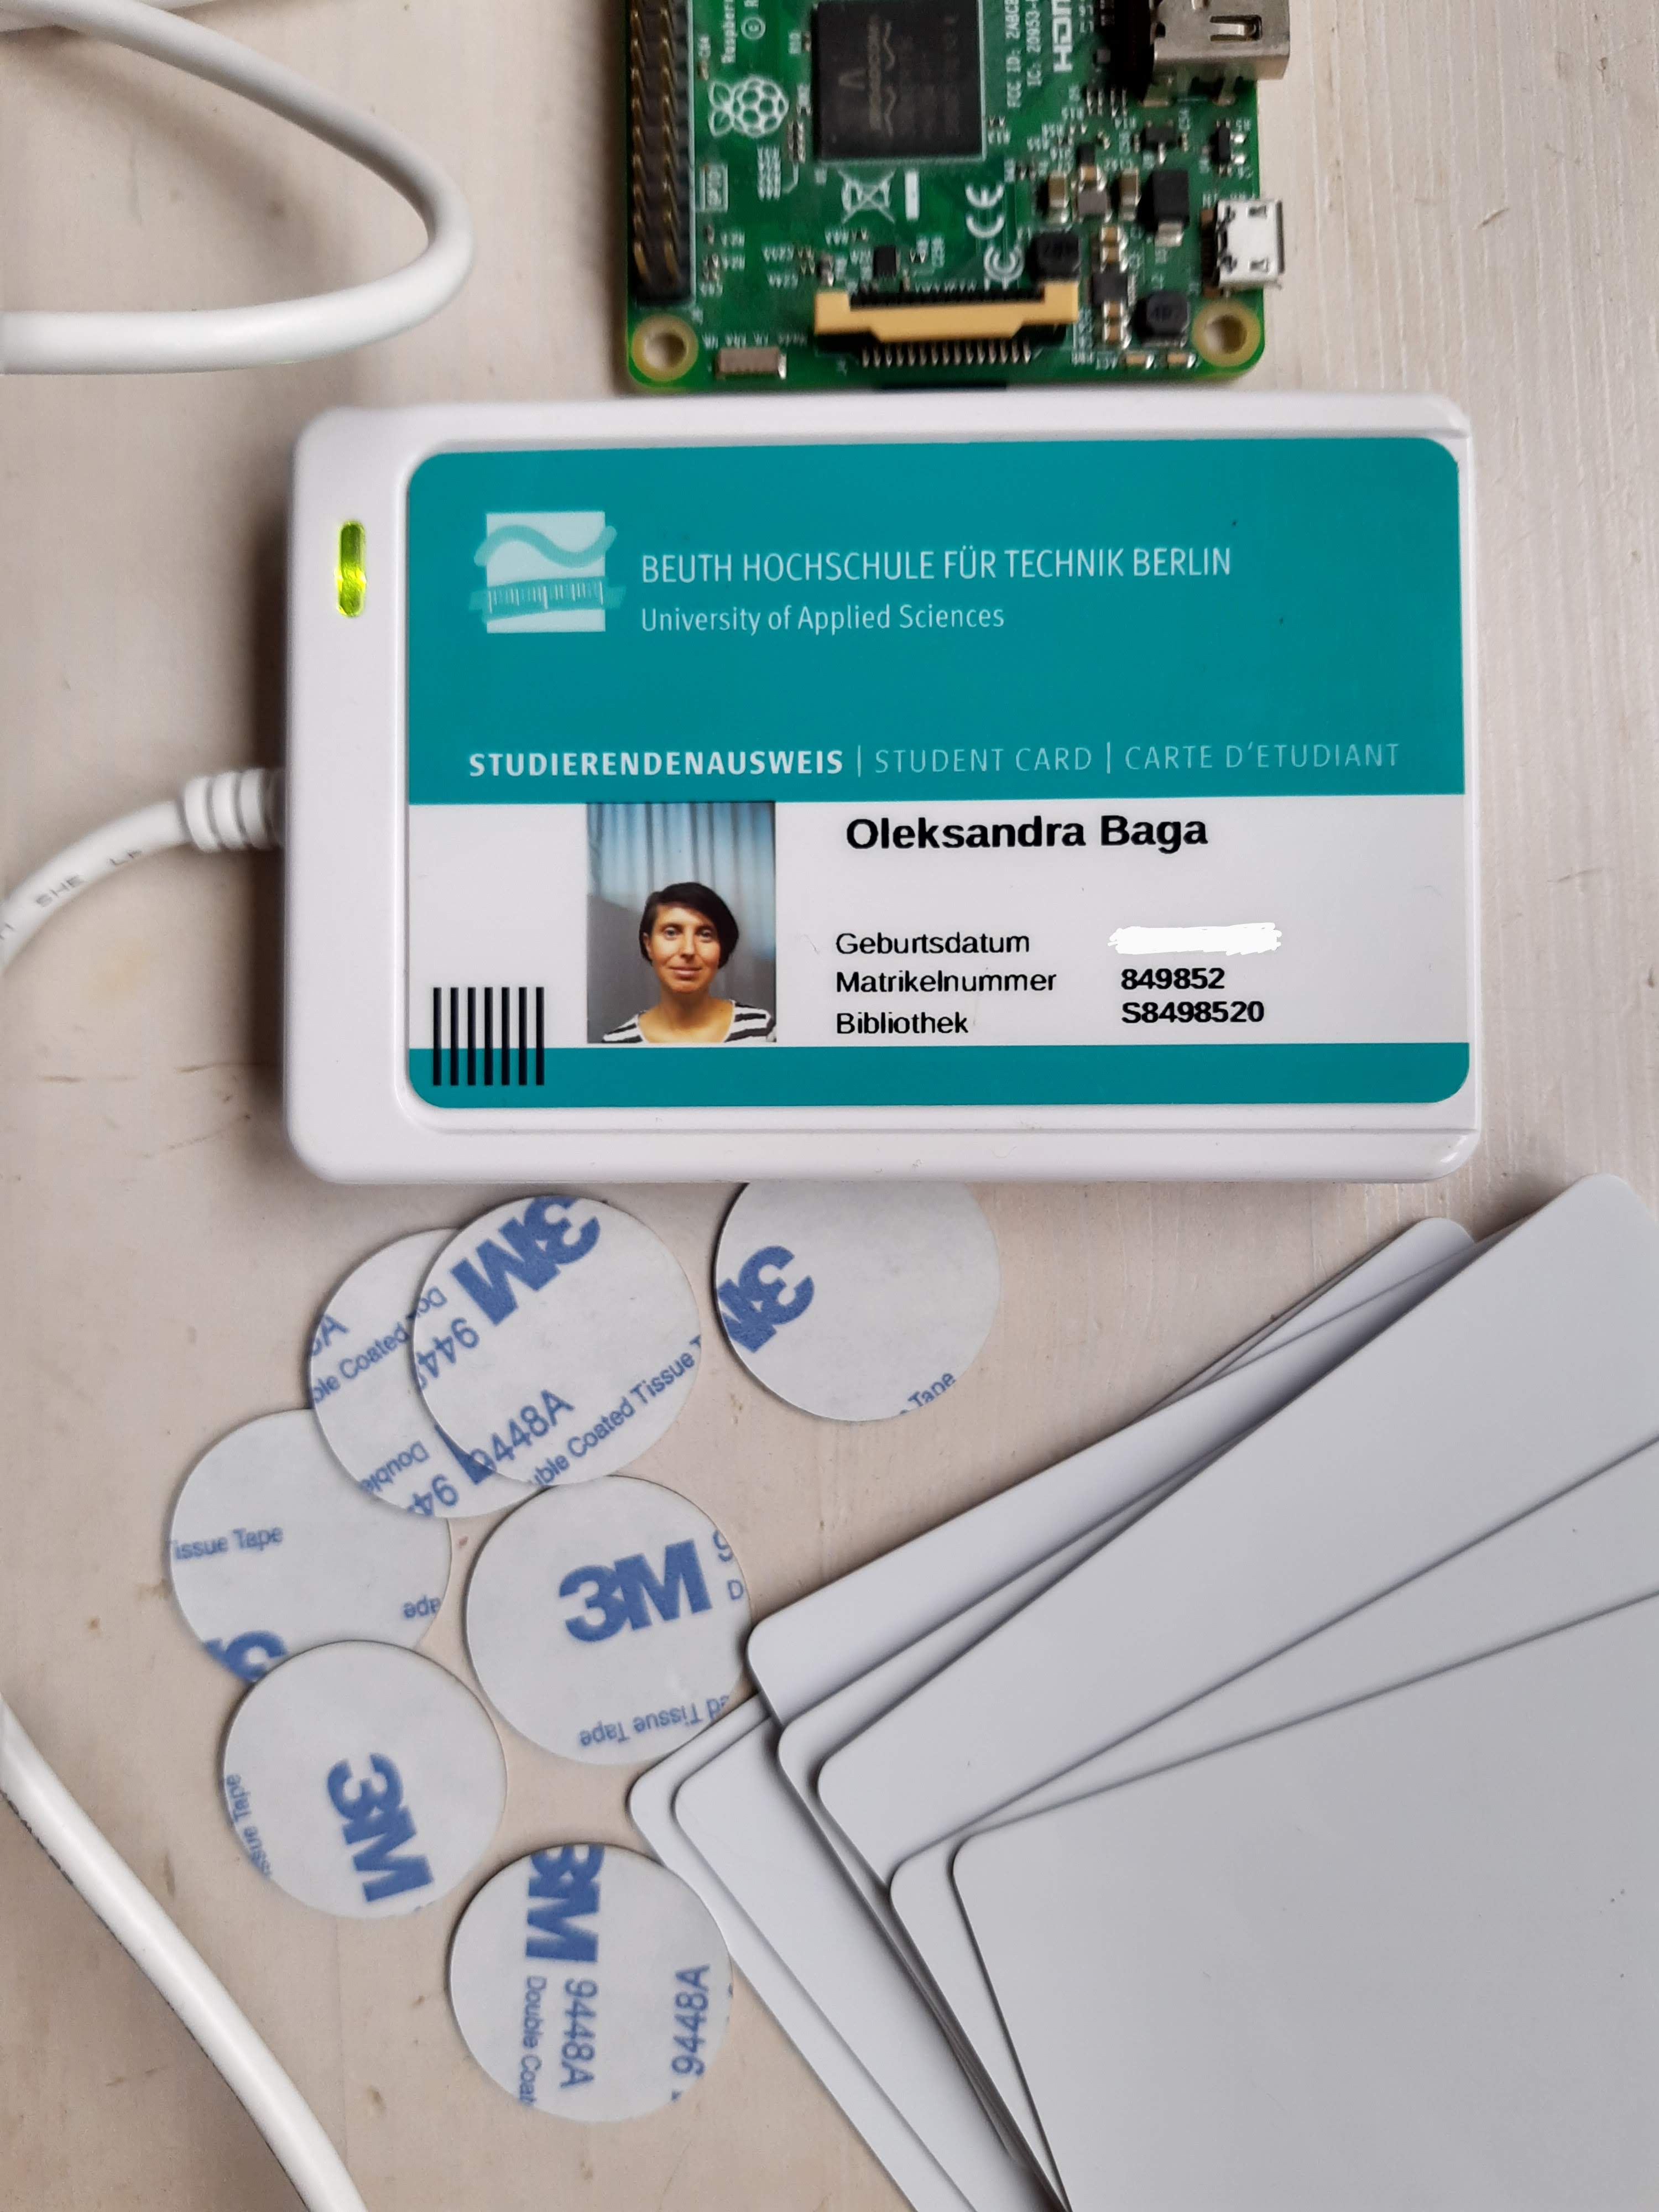
\includegraphics[width=0.42\textwidth]{gfx/baga_stud.jpg}}
	\caption{RFID-Leser mit der Studentenkarte der Autorin und RFID-Transponders}
	\label{fig:baga_stud}
\end{wrapfigure} 
Wie die weitere Entwicklung darf einfach den ersten gefundenen RFID-Leser genommen werden. Wenn keine Terminals angeschlossen sind, wird das Programm beendet und eine entsprechende Meldung der PSE-Labor Mitarbeiter ausgegeben. Dann muss mit dem ausgewählten Terminal verbunden werden. Dies erfolgt durch Aufrufen der Funktion $SCardConnect()$. Beim Aufruf von $SCardConnect()$ geben wir den gemeinsam genutzten Modus $(SHARE\_SHARED)$, das bevorzugte Kommunikationsprotokoll (in unserem Fall T0 und T1) an, übergeben die Adresse der Variablen, in die das Handle für weitere Operationen mit der Karte gespeichert wird, und die Adresse der Variablen $active\_protocol$. in der gewählten Kommunikationsprotokoll gespeichert wird. Auf Anwendungsebene interessiert es uns nicht besonders, welches Protokoll zum Herstellen der Verbindung ausgewählt wurde, aber diese Informationen müssen während der Programmierung gespeichert werden - sie werden später zum Senden von Befehlen benötigt\cite[p. 104]{chirico:smart_card}.
\begin{lstlisting}
hresult, hcontext = SCardEstablishContext(SCARD_SCOPE_USER)
	if hresult == SCARD_S_SUCCESS:
		hresult, readers = SCardListReaders(hcontext, [])
		if len(readers) > 0:
			reader = readers[0]
			hresult, hcard, dwActiveProtocol = SCardConnect(hcontext, reader, SCARD_SHARE_SHARED, SCARD_PROTOCOL_T0 | SCARD_PROTOCOL_T1)
\end{lstlisting}

ATR (Answer-To-Reset) ist ein kurzes (nicht mehr als 33) Byte-Array, das die Karte beim Anschließen an das Terminal senden muss. Wenn die Karte dies nicht innerhalb einer bestimmten Zeit tut, wird davon ausgegangen, dass sie nicht richtig funktioniert. ATR enthält grundlegende Informationen über die Karte und die technischen Parameter der Verbindung. Das Format ist jedoch recht kompliziert und hängt vom Hersteller des Kartenchips, den darauf installierten „Anwendungen“ usw. ab. ATR wird im Terminal gespeichert, solange die Karte angeschlossen ist. Es lässt sich die zwei verschiedenen RFID-Transponder (MIFARE Smart-Studentenkarte und RFID-Tag) mit Hilfe ATR voneinander unterscheiden. Das folgendes wird z.B. von der Studentenkarte zurückbekommen, wann Autorin ihre eigene Studentenkarte am RFID-Leser ablesen lässt (siehe Abbildung \ref{fig:baga_stud}):
\begin{lstlisting}
+Inserted:  3B 81 80 01 80 80
Student card added
uid 04 2F 75 7A 30 40 80
\end{lstlisting}

Das anderes wird aber angezeigt, wann den RFID-Transponder am RFID-Leser präsentiert wird, den in der Zukunft am im PSE-Labor vorhandenen Raspi-Boards angeklebt wird:
\begin{lstlisting}
+Inserted:  3B8F8001804F0CA000000306030001000000006A
Raspi board added
uid 5C E7 87 30
\end{lstlisting}

Klasse $DetectionObserver$ mit der Vererbung vom der Klasse $CardObserver$ wird benutzt, um zu erkennen, wann eine Karte dem Kartenleser vorgelegt wurde, und dann die eindeutige Kennung (UID) von einer Karte zu lesen. Es wird mithilfe der Klasse $ CardMonitor$ getan, die das Einsetzen / Entfernen von Smartcards überwacht und den $CardObserver$ benachrichtigt. 
\begin{lstlisting}[language=Python]
def update(self, observable, actions):
	(addedcards, removedcards) = actions
	for card in addedcards:
		atr = toHexString(card.atr)
		added_card = self.get_cardtype(toHexString(card.atr), "added")
		self.read_uid(added_card)
\end{lstlisting}

Sobald eine korrekte Studentenkarte oder RFID-Transponder am RFID-Leser erscheint und ohne Kollision mit anderen in der Nähe bleibenden elektromagnetische Felde abgelesen wird, wird abhängig vom dem Typ der Karte eine JSON-Datei erstellt und von einem acaLoan-client zum Server geschickt. Der acaLoan-client selbst ist ein kleinen Python-Script, der die korrekte Erstellung der JSON-Datei erlaubt und eine Verbindung mittels HTTP-Protokoll zum Server bedient. 
\begin{lstlisting}
class AcaLoanClient:
	def __init__(self, base_url):
		self.base_url = base_url
	
	def send_event(self, type, uid):
		endpoint = "{}/loan/api/events".format(self.base_url)
		payload = {"type": type, "uid": uid}
		r = requests.post(endpoint, json=payload)
\end{lstlisting}

Es wird weiteres von Register-Client auf keine Antwort vom Server erwartet, ob der abgelesenen Studentenkarte die Ausleihe des Raspi-Boards erlaubt ist oder ob gehaltenen in der Hand Raspi-Board ausgeliehen oder zurückgegeben darf. Sobald die Verbindung zum Server erfolgreich hergestellt wurde und eine JSON-Datei geschickt, wird der RFID-Leser wieder zum Ablesen der nächsten RFID-Transponder freigegeben. Der Python-Script für RFID-Leser muss am Register-Client mit der Verwendung der Umgebungsvariable $LOAN_SERVER$. Während der Entwicklung der Abschlussarbeit geschieht es mit dem Name des Django Entwicklungsservers. Mehr darüber ist in folgenden Kapitel \ref{sec:server} nachzulesen.
\begin{lstlisting}
LOAN_SERVER_URL=http://127.0.0.1:8000 python reader.py
\end{lstlisting}
Als letztes für die Implementierung des Register-Clients ist es wichtig, die kurze Beschreibung der entwickelte von Autorin JSON-Datei anzugeben. Definition der Struktur, des Inhalts und der Semantik von JSON-Objekten geschieht mithilfe von der Grammatiksprache namens JSON-Schema. Hier kann Metadaten (Daten über die Daten) angegeben werden, die die Eigenschaften eines Objekts beschreiben und gültige Werte. 

\begin{lstlisting}
{"$schema": "http://json-schema.org/draft-04/schema#",
"type": "array", "items": [
	{"type": "object", "properties": {
		"type": {"type": "string",
			"enum": ["card", "uid", "cancel_button", "terminate_button", "get_rfid_status",
			"return_scanned_board_button", "loan_scanned_board_button", "finish_button"]},
		"uid": {"type": "string"}},
	"required": ["type", "uid"]}]}
\end{lstlisting}

Zu Zweck Definition der Struktur wird das Schlüsselwort "items" mit einem Array gesetzt, wobei jedes Element ein Schema ist, das jedem Index des Arrays des Dokuments entspricht. Das heißt, ein Array, bei dem das erste Element das erste Element des Eingabearrays validiert, das zweite Element das zweite Element des Eingabearrays validiert usw\cite{website:14}. Es ist zu betonen, dass für das ersten Element der JSON-Datei es eine Zeichenfolge aus einem festen Wertesatz sein muss. Nur diesen Zeichenfolgen können von Endliche Zustandsmaschine, die im Kapitels \ref{sec:design:fsm} und \ref{sec:server:restapi} beschrieben sind, abgearbeitet werden. 

\section{Server}
\label{sec:server}
Als er wurde im Kapitel \ref{sec:register_client:smart} erwähnt, während der Implementierung der Aufgabe der Abschlussarbeit wurde mit dem Entwicklungsserver gearbeitet. Ein Entwicklungsserver ist ein Servertyp, der die Entwicklung und das Testen von Programmen, Websites, Software oder Anwendungen für Softwareprogrammierer erleichtert. Der bietet eine Laufzeitumgebung sowie alle Hardware- / Software-Dienstprogramme, die für das Debuggen und die Entwicklung von Programmen unerlässlich sind. Django ist eines der effizientesten modernen Frameworks für die Entwicklung von Webprojekten. Der Grund für diese Effizienz ist ein klarer Mechanismus für die Arbeit mit einem Projekt, ein praktisches ORM (Object Relational Mapping Layer), mit der mit Anwendungsdaten aus verschiedenen relationalen Datenbanken wie SQLite, PostgreSQL und MySQL interagiert werden kann.

\subsection{Erstellung acaLoan Django-Projekts}
\label{sec:server:install}
Glücklicherweise ist der Installationsprozess für Django unkompliziert, sodass das Einrichten Ihrer Entwicklungsumgebung schnell und entspannt ist. Django ist vollständig in Python geschrieben, daher muss zuerst Python installiert werden, um Django zu installieren. Weil die Autorin für die Implementierung des Servers ihren eignen Mac OS Rechner verwendet, ist Python bereits Computer installiert. Wenn "Python" in die Befehlszeile eingegeben (mithilfe der Terminal.app auf meinem Mac), wurde folgendes angezeigt werden:
\begin{lstlisting}
$ python
Python 3.8.1 (default, Feb 17 2020, 23:55:16) 
[Clang 11.0.0 (clang-1100.0.33.17)] on darwin
\end{lstlisting}

Sobald Python auf Computer installiert ist, kann Django auch installiert werden. Es gibt drei Möglichkeiten: Installation der offizielle Django-Version, Verwendung eines verteilungsspezifisches Installationsprogramm oder Herunterladen der Version, die derzeit immer noch entwickelt wird. In der Abschlussarbeit wird nur die Installation der offiziellen Version verwendet. Der Installation wird mit "Pipenv"-Tool geschieht, das isolierte Python-Umgebungen bietet, die somit praktischer sind als die systemweite Installation von Paketen. Pipenv verwaltet Projektpakete automatisch über die Pipfile-Datei, während die Pakete installiert oder deinstalliert werden. Pipenv generiert auch die Datei Pipfile.lock, mit der deterministische Builds erstellt und eine Momentaufnahme Ihrer Arbeitsumgebung erstellt werden. Zusätzlich für die Aufgabeimplementierung wird django-fsm installiert, das mit der Django Installation nicht geliefert wird und erlaubt eine einfache deklarative Zustandsverwaltung für Django-Modelle. 

Der ganzen Quellcode für das acaLoan-Server wird als Django Projekt dargestellt. Django hat einen Befehl zum einfachen Erstellen einer anfänglichen Projektstruktur. Es wird mit der Ausführung des folgenden Befehls vom Terminal erledigt:
\begin{lstlisting}
 django-admin startproject acaLoanRaspiBoard   
\end{lstlisting}

\begin{figure}
	\centering
	\fbox{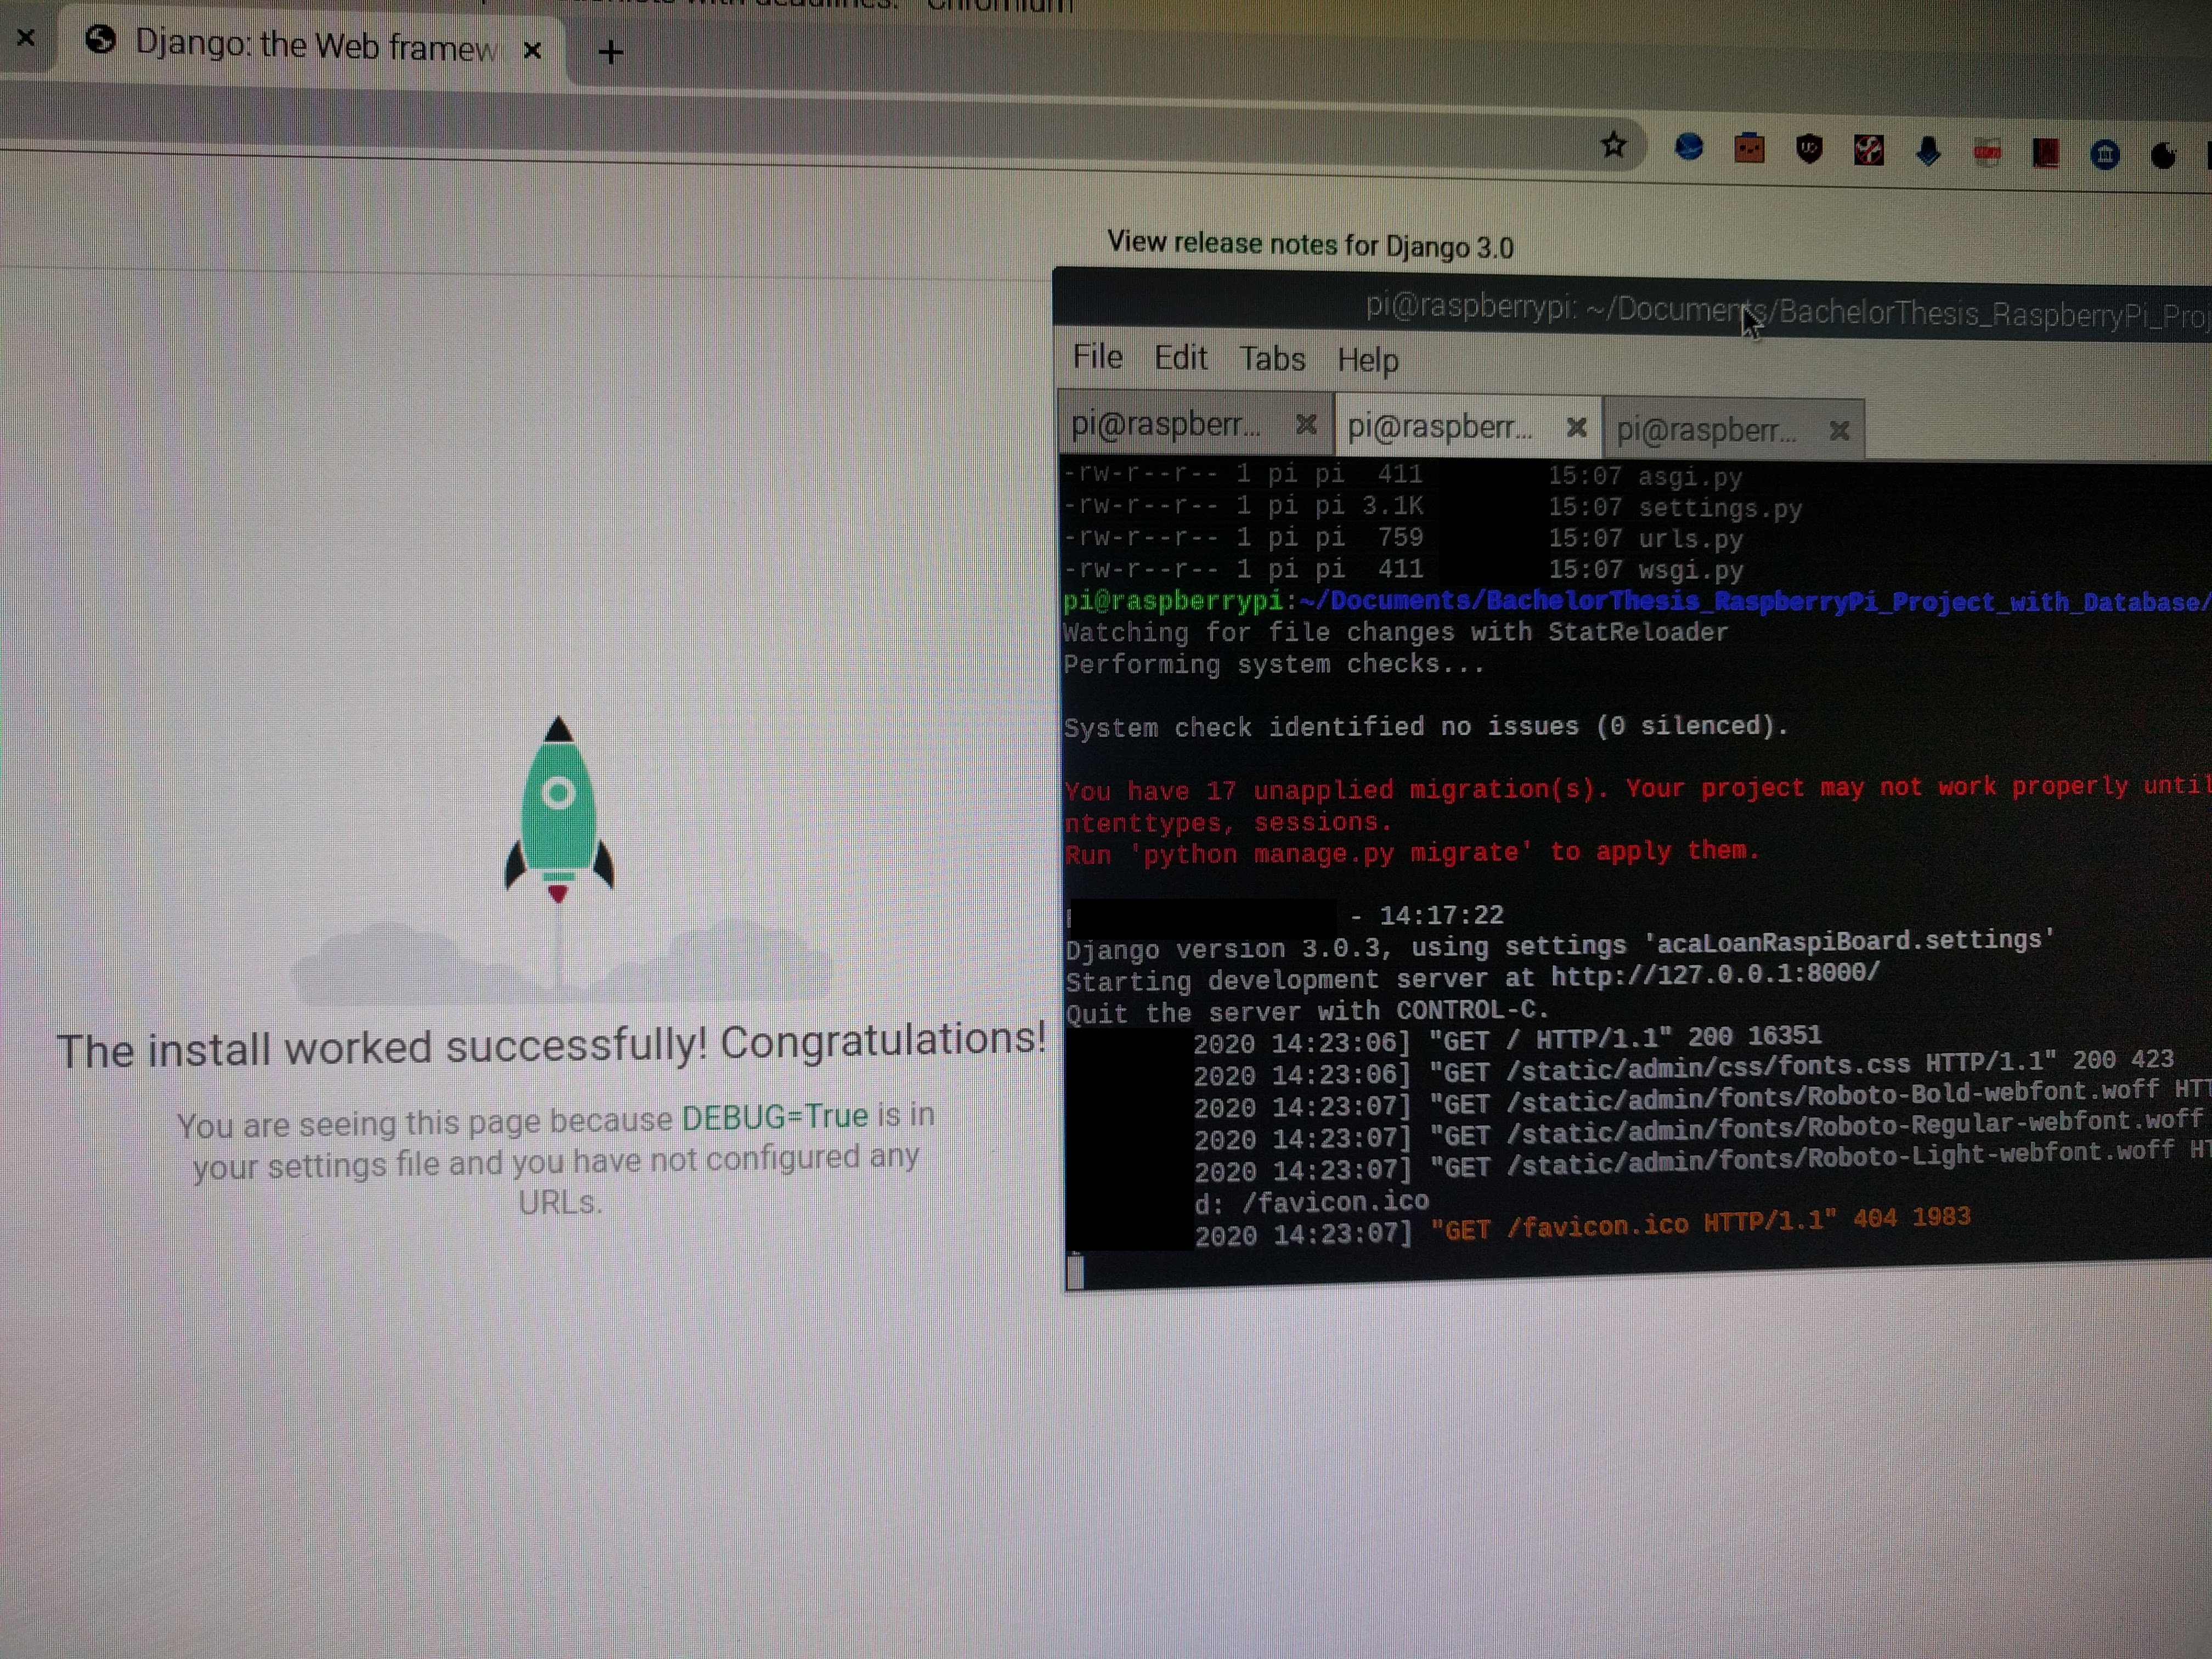
\includegraphics[width=1\textwidth]{gfx/django_start.jpg}}
	\caption{Screenshot von Raspberry Pi nach dem Erstellung des acaLoanRaspiBoard-Projekts.}
	\label{fig:django_start}
\end{figure}

Die Datei settings.py enthält eine Grundkonfiguration für die Verwendung einer SQLite-Datenbank und eine Liste von Django-Anwendungen und wurde als während der Implementierung geändert, um das üblichste deutsche Zeitformat anstatt des amerikanischen zu verwenden.
\begin{lstlisting}[caption={My Caption},captionpos=b]
LANGUAGE_CODE = 'en-us'
TIME_ZONE = 'Europe/Berlin'
TIME_INPUT_FORMATS = ['%H:%M:%S']
TIME_FORMAT = '%H:%M:%S'
DATETIME_FORMAT = "d.m.Y H:m"
DATE_FORMAT = "Y-m-d"
\end{lstlisting}
acaLoan-Server muss im zusätzliche Dateien wie Bilder, JavaScript oder CSS bereitstellen. In Django werden diese Dateien als "statische Dateien" bezeichnet. Django stellt django.contrib.staticfiles zur Verfügung, um den Entwickler bei der Verwaltung zu unterstützen. Dafür müssen in die Datei settings.py die folgenden Zeilen hinzugefügt werden:
\begin{lstlisting}
STATIC_URL = '/static/'
STATICFILES_DIRS = [os.path.join(BASE_DIR, "staticfiles")]
\end{lstlisting}

In der settings.py ist auch den Debug-Modus des Projekts aktiviert, um während der Entwicklung detaillierte Fehlermeldungen zu sehen.  Nach der Erstellung des Projekts und kleine notwendigen Änderungen, kann endlich acaLoan-Server gestartet werden. Da Django einen praktischen Mechanismus bietet, um die Konfiguration Ihres Webservers während der Entwicklung zu vermeiden, kann enthaltenen bereits ein Webserver mit dem Befehl aufgerufen werden: 
\begin{lstlisting}
python manage.py runserver
\end{lstlisting}
Nach dem Befehl ausgeführt wurde und im Browser zu http://127.0.0.1:8000/ navigiert wurde, wird die folgende Ausgabe angezeigt, die auf der Abbildung \ref{fig:django_start} zu sehen ist.
 
\subsection{Datenbankeinrichtung}
\label{sec:server:database}
Nach dem Erstellung des Projekts und dem ersten Starten des acaLoan-Server ist es die Zeit, sich mit der Einrichtung von Datenbank zu beschäftigen. Theoretisch kann ein Django-basierte Projekt ohne Datenbank ausgeführt werden. Für die hier vorliegenden Abschlussarbeit was jedoch es ein Zweck, eine Datenbank einzurichten, um alle Ausleihe-/Rückgabevorgänge zu verwalten, so dass in einem echten Projekt kann man nicht auf Datenbankeinrichtung verzichten. Für die Implementierung wird für Verwendung von SQLite3 entschieden. Die Datenbank selbst wird in einer Datei auf der Festplatte gespeichert. Um die Datenbank mit dem Django-Projekt zu verbinden, muss den DATABASES-Block in der Datei $mysite/settings.py$ bearbeitet. Um sqlite zu verwenden, muss nur $django.db.backends.sqlite3$ als ENGINE angegeben und den Namen der Datei, in der die Datenbank gespeichert wird, in den Parameter NAME geschrieben werden\cite{website:15}.

Als nächsten müssen die Modelle in Django erzeugt werden, die die Daten definieren, mit denen während der Entwicklung gearbeitet werden. Die Modelle in Django werden entsprechend des Entity Relationship Diagrams realisiert, das im Kapitel \ref{sec:design:db} gezeigt wurde. Die wichtigste Modelle sind unten zu sehen:

\begin{lstlisting}
class Student(models.Model):
	student_card = models.OneToOneField(StudentCard, on_delete=models.SET_NULL, blank=True, null=True)
	semester = models.ForeignKey(Semester, on_delete=models.CASCADE, blank=True, null=True)
	first_name = models.CharField('first name', max_length=50)
	second_name = models.CharField('second name', max_length=50)
	matricul_no = models.CharField('matriculation', max_length=10, unique=True)
	hrz_no = models.CharField('hrz', max_length=10, unique=True)
	group = enum.EnumField(StudentGroup)
	is_home_loan_enabled = models.BooleanField(default=True)
\end{lstlisting}
 ForeignKey wird verwendet, um eine Viele-zu-Eins-Beziehung zu definieren, die eine Beziehung zwischen mehr als einer Instanz einer Entität und einer Instanz einer anderen Entität ist. Sodass in der Datenbank für ein Semester können mehrere Studierende immatrikuliert werden.
 \begin{lstlisting}
 content...
 \end{lstlisting}

\subsection{Erstellen der öffentlichen Schnittstelle - "Views"}
\label{sec:server:views}

\subsection{Einführung in das Django Admin}
\label{sec:server:admin}

\subsection{Templates und Design der acaLoan-Website}
\label{sec:server:design}

\subsection{Implementierung des Anwendungsfällen}
\label{sec:server:fsm}
Während der Implementierung der User Cases wurde auch Sequenzdiagramm erzeugt, die einfach die Interaktionen zwischen Objekten in einer sequentiellen Reihenfolge zeigt, d.h. die Reihenfolge, in der diese Wechselwirkungen stattfinden. Die Sequenzdiagramm wurde als nächstes als eine Basis für das Design des Zustandsmaschine verwendet.  

\subsubsection{Sequenzdiagramm}
\label{sec:server:fsm:sequenz}
\begin{figure}
	\centering
	\fbox{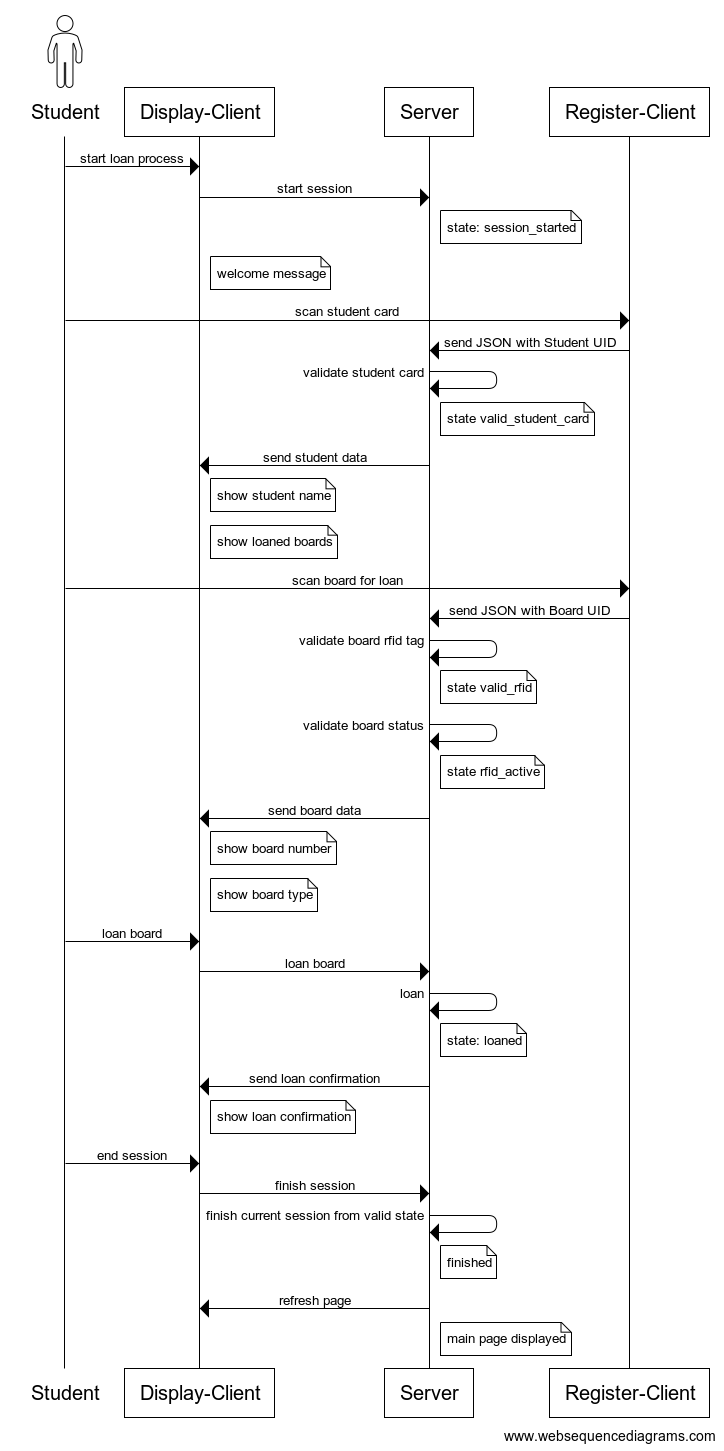
\includegraphics[width=0.8\textwidth]{gfx/seq.png}}
	\caption{Sequenzdiagramm der erfolgreichen Ausleihe der Lab-Loan Raspi Board}
	\label{fig:seq}
\end{figure}
Ein Sequenzdiagramm beschreiben, wie und in welcher Reihenfolge die Objekte in einem System funktionieren. In der Abschlussarbeit werden ein Sequenzdiagramm gezeigt, die auf den Abbildungen \ref{fig:seq} zu betrachten ist. Es ist ein erfolgreichen Szenario für die Ausleihe der Lab-Loan Raspi Board von einem gültigen Studierende. Das Sequenzdiagramme entspricht der oben genannte User Story \textit{"As a student, I want to loan a board so I can work at lab"}. Die meisten Kommunikation geschieht über die asynchrone Nachrichten. Zum Beispiel, es wird von Register-Klient mit dem angeschlossenen RFID-Leser nicht darauf gewartet, ob die abgelesene Studentenkarte gültig ist oder ob ein Student zum Kurs zugelassen ist. Sofort die vorherigen Ablesevorgang angeschlossen wurde und JSON-Datei dem Server geschickt, steht der RFID-Leser wieder zur Verfügung und ein RFID-Tag des Boards abgelesen werden kann. Es kann sogar sein, dass anstatt erwarteten in erfolgreichen Szenario RFID-Tags eine weitere Studentenkarte abgelesen wird (z.B. nebenstehende Kumpel der Studierende aus Spaß oder wegen der Eile lässt seine Karte ablesen vor dem Beenden des laufenden Ausleihevorgang). Obwohl es aus der Sich der Zustandsmaschine nicht zugelassen ist, eine weitere Studentenkarte zu lesen, wird trotzdem die Karte von RFID-Reader abgelesen, eine weitere JSON-Datei zum Server geschickt und weiter RFID-Leser zum nächsten Lesen freigegeben. Es ist rein die Aufgabe des Servers die ankommenden Daten zu verifizieren und den Zustandsmaschine in einem weiteren Zustand zu schalten. Die entsprechende Information mit der Begrüßung der Studierende oder Fehlermeldung wird auch vom Server generiert und dem Display-Client zum Anzeigen übergeben. Mehr über diese Vorgehensweise in entsprechenden Kapitels \ref{sec:register_client:smart}, \ref{sec:server:fsm} und \ref*{sec:display_client:js} der Implementierungsphase nachzulesen. 

\subsubsection{Endliche Zustandsmaschine mit Django FSM}
\label{sec:server:fsm:fsm}


\section{Display-Client}
\label{sec:display_client}

\subsection{Clientseitiges JavaScript}
\label{sec:display_client:js}


\section{Automatisierten Tests}
\label{sec:testing}